\documentclass[11pt,preprint, authoryear]{elsarticle}

\usepackage{lmodern}
%%%% My spacing
\usepackage{setspace}
\setstretch{1.2}
\DeclareMathSizes{12}{14}{10}{10}

% Wrap around which gives all figures included the [H] command, or places it "here". This can be tedious to code in Rmarkdown.
\usepackage{float}
\let\origfigure\figure
\let\endorigfigure\endfigure
\renewenvironment{figure}[1][2] {
    \expandafter\origfigure\expandafter[H]
} {
    \endorigfigure
}

\let\origtable\table
\let\endorigtable\endtable
\renewenvironment{table}[1][2] {
    \expandafter\origtable\expandafter[H]
} {
    \endorigtable
}


\usepackage{ifxetex,ifluatex}
\usepackage{fixltx2e} % provides \textsubscript
\ifnum 0\ifxetex 1\fi\ifluatex 1\fi=0 % if pdftex
  \usepackage[T1]{fontenc}
  \usepackage[utf8]{inputenc}
\else % if luatex or xelatex
  \ifxetex
    \usepackage{mathspec}
    \usepackage{xltxtra,xunicode}
  \else
    \usepackage{fontspec}
  \fi
  \defaultfontfeatures{Mapping=tex-text,Scale=MatchLowercase}
  \newcommand{\euro}{€}
\fi

\usepackage{amssymb, amsmath, amsthm, amsfonts}

\def\bibsection{\section*{References}} %%% Make "References" appear before bibliography


\usepackage[round]{natbib}

\usepackage{longtable}
\usepackage[margin=2.3cm,bottom=2cm,top=2.5cm, includefoot]{geometry}
\usepackage{fancyhdr}
\usepackage[bottom, hang, flushmargin]{footmisc}
\usepackage{graphicx}
\numberwithin{equation}{section}
\numberwithin{figure}{section}
\numberwithin{table}{section}
\setlength{\parindent}{0cm}
\setlength{\parskip}{1.3ex plus 0.5ex minus 0.3ex}
\usepackage{textcomp}
\renewcommand{\headrulewidth}{0.2pt}
\renewcommand{\footrulewidth}{0.3pt}

\usepackage{array}
\newcolumntype{x}[1]{>{\centering\arraybackslash\hspace{0pt}}p{#1}}

%%%%  Remove the "preprint submitted to" part. Don't worry about this either, it just looks better without it:
\makeatletter
\def\ps@pprintTitle{%
  \let\@oddhead\@empty
  \let\@evenhead\@empty
  \let\@oddfoot\@empty
  \let\@evenfoot\@oddfoot
}
\makeatother

 \def\tightlist{} % This allows for subbullets!

\usepackage{hyperref}
\hypersetup{breaklinks=true,
            bookmarks=true,
            colorlinks=true,
            citecolor=blue,
            urlcolor=blue,
            linkcolor=blue,
            pdfborder={0 0 0}}


% The following packages allow huxtable to work:
\usepackage{siunitx}
\usepackage{multirow}
\usepackage{hhline}
\usepackage{calc}
\usepackage{tabularx}
\usepackage{booktabs}
\usepackage{caption}


\newenvironment{columns}[1][]{}{}

\newenvironment{column}[1]{\begin{minipage}{#1}\ignorespaces}{%
\end{minipage}
\ifhmode\unskip\fi
\aftergroup\useignorespacesandallpars}

\def\useignorespacesandallpars#1\ignorespaces\fi{%
#1\fi\ignorespacesandallpars}

\makeatletter
\def\ignorespacesandallpars{%
  \@ifnextchar\par
    {\expandafter\ignorespacesandallpars\@gobble}%
    {}%
}
\makeatother

\newenvironment{CSLReferences}[2]{%
}

\urlstyle{same}  % don't use monospace font for urls
\setlength{\parindent}{0pt}
\setlength{\parskip}{6pt plus 2pt minus 1pt}
\setlength{\emergencystretch}{3em}  % prevent overfull lines
\setcounter{secnumdepth}{5}

%%% Use protect on footnotes to avoid problems with footnotes in titles
\let\rmarkdownfootnote\footnote%
\def\footnote{\protect\rmarkdownfootnote}
\IfFileExists{upquote.sty}{\usepackage{upquote}}{}

%%% Include extra packages specified by user
\usepackage{booktabs}
\usepackage{longtable}
\usepackage{array}
\usepackage{multirow}
\usepackage{wrapfig}
\usepackage{float}
\usepackage{colortbl}
\usepackage{pdflscape}
\usepackage{tabu}
\usepackage{threeparttable}
\usepackage{threeparttablex}
\usepackage[normalem]{ulem}
\usepackage{makecell}
\usepackage{xcolor}

%%% Hard setting column skips for reports - this ensures greater consistency and control over the length settings in the document.
%% page layout
%% paragraphs
\setlength{\baselineskip}{12pt plus 0pt minus 0pt}
\setlength{\parskip}{12pt plus 0pt minus 0pt}
\setlength{\parindent}{0pt plus 0pt minus 0pt}
%% floats
\setlength{\floatsep}{12pt plus 0 pt minus 0pt}
\setlength{\textfloatsep}{20pt plus 0pt minus 0pt}
\setlength{\intextsep}{14pt plus 0pt minus 0pt}
\setlength{\dbltextfloatsep}{20pt plus 0pt minus 0pt}
\setlength{\dblfloatsep}{14pt plus 0pt minus 0pt}
%% maths
\setlength{\abovedisplayskip}{12pt plus 0pt minus 0pt}
\setlength{\belowdisplayskip}{12pt plus 0pt minus 0pt}
%% lists
\setlength{\topsep}{10pt plus 0pt minus 0pt}
\setlength{\partopsep}{3pt plus 0pt minus 0pt}
\setlength{\itemsep}{5pt plus 0pt minus 0pt}
\setlength{\labelsep}{8mm plus 0mm minus 0mm}
\setlength{\parsep}{\the\parskip}
\setlength{\listparindent}{\the\parindent}
%% verbatim
\setlength{\fboxsep}{5pt plus 0pt minus 0pt}



\begin{document}



\begin{frontmatter}  %

\title{Predicting Employee Attrition}

% Set to FALSE if wanting to remove title (for submission)




\author[Add1]{Hannah MacGinty}
\ead{21082022@sun.ac.za}





\address[Add1]{Stellenbosch University, South Africa}


\begin{abstract}
\small{
This paper investigates employee attributes and attrition. Predictive
models for employee attrition are built based on key attributes, such as
education, pay, gender, and age, among others. After assessing logistic,
K-Nearest Neighbours and Random Forest models, a tuned random forest
model is found to be the best predictor of this particular
classification problem due to its high accuracy rates and good
performance on unseen data.
}
\end{abstract}

\vspace{1cm}





\vspace{0.5cm}

\end{frontmatter}

\setcounter{footnote}{0}



%________________________
% Header and Footers
%%%%%%%%%%%%%%%%%%%%%%%%%%%%%%%%%
\pagestyle{fancy}
\chead{}
\rhead{}
\lfoot{}
\rfoot{\footnotesize Page \thepage}
\lhead{}
%\rfoot{\footnotesize Page \thepage } % "e.g. Page 2"
\cfoot{}

%\setlength\headheight{30pt}
%%%%%%%%%%%%%%%%%%%%%%%%%%%%%%%%%
%________________________

\headsep 35pt % So that header does not go over title




\hypertarget{introduction}{%
\section*{Introduction}\label{introduction}}
\addcontentsline{toc}{section}{Introduction}

Losing employees can be costly for businesses. Predicting attrition and
its key determinants or attributes can help estimate future employee
turnover and consequently help companies attempt to reduce it. This
paper compares various models in an attempt to predict employee
attrition from a company-wide dataset on 4653 employees. After exploring
the data, a logistic model is estimated and predictions across training
and test data are conducted. Following this, predictions are generated
from an optimised K-Nearest Neighbours model. Lastly, random forest
models are investigated in an attempt to find the best predictive model
for the classifcation problem at hand.

\hypertarget{exploratory-data-analaysis}{%
\section*{Exploratory Data Analaysis}\label{exploratory-data-analaysis}}
\addcontentsline{toc}{section}{Exploratory Data Analaysis}

The dataset contains information on 4653 employees and whether they left
their job or not. A variety of employee attributes are available,
including demographic information such as age and gender. Employees are
based in one of three major cities in India, namely Bangalore, Pune and
New Delhi. The year an employee joined a company, ranging from 2014 to
2018, is also considered.

Given that earnings are generally an important determinant in whether an
employee leaves their job, their payment tier, scaled from 1, being the
highest, and 3, being the lowest, is included in the data. Additionally,
years of experience in their current field is included as well as their
highest level of education (Bachelor's, Master's, PhD). There is also
information on whether an employee kept out of projects for 1 month or
more, which could potentially indicates an employee's lack of interest
in work or plans to leave the company.

On examination of the spread of employees across cities, most of the
employees are from Bangalore. Regarding education level, most employees
have a Bachelors degree. Only 179 employees have a PHD and 873 have
Master's degrees.

\begin{figure}[H]

{\centering 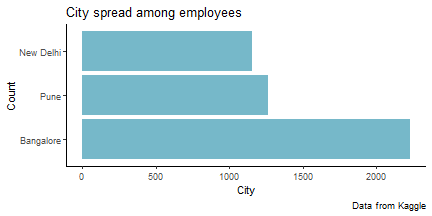
\includegraphics{Final_project_files/figure-latex/Figure1-1} 

}

\caption{City Spread \label{Figure1}}\label{fig:Figure1}
\end{figure}

\begin{figure}[H]

{\centering 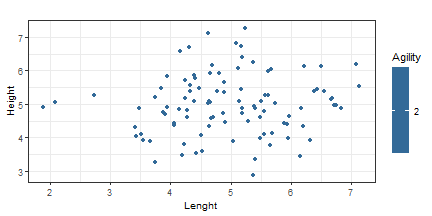
\includegraphics{Final_project_files/figure-latex/Figure2-1} 

}

\caption{Education Spread \label{Figure2}}\label{fig:Figure2}
\end{figure}

Looking at age, which ranges between 22 and 41, the majority of
employees are in their mid to late twenties, skewing the distribution to
right.

Regarding experience, very few individuals have 6 or 7 years experience
(only 16 employees in total) in their current field of work, most likely
due to the young employee base. Most commonly, individuals have 2 years
experience.

2017 saw the most employees join the company. There was a substantial
fall in employees joining in 2018. Only 367 employees joined in 2018,
compared to 1180 in 2017.

\begin{figure}[H]

{\centering 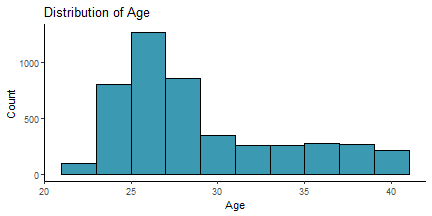
\includegraphics{Final_project_files/figure-latex/Figure3-1} 

}

\caption{Age Distribution \label{Figure3}}\label{fig:Figure3}
\end{figure}

\begin{figure}[H]

{\centering 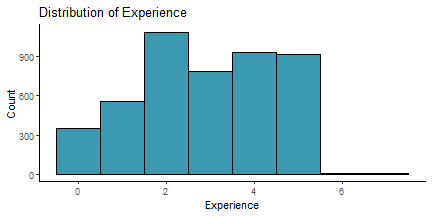
\includegraphics{Final_project_files/figure-latex/Figure4-1} 

}

\caption{Experience Distribution \label{Figure4}}\label{fig:Figure4}
\end{figure}

\begin{figure}[H]

{\centering 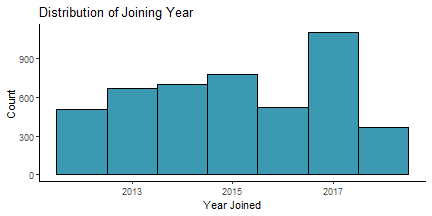
\includegraphics{Final_project_files/figure-latex/Figure5-1} 

}

\caption{Joining Year Distribution \label{Figure5}}\label{fig:Figure5}
\end{figure}

Attrition rates are highest among those with Master's degrees. Nearly
fifty percent of those with Master's degrees left their job. When
looking across joining year, almost all the employees that joined in
2018 resigned. It is possible that some event occurred in 2018 that
caused that cohort to subsequently leave.

\begin{figure}[H]

{\centering 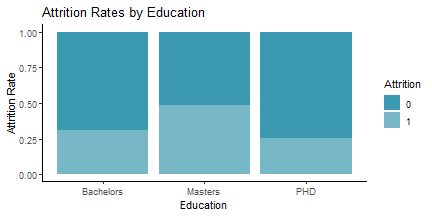
\includegraphics{Final_project_files/figure-latex/Figure6-1} 

}

\caption{Attrition by Education \label{Figure6}}\label{fig:Figure6}
\end{figure}

\begin{figure}[H]

{\centering 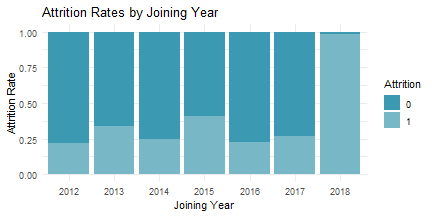
\includegraphics{Final_project_files/figure-latex/Figure7-1} 

}

\caption{Attrition by Joining Year \label{Figure7}}\label{fig:Figure7}
\end{figure}

The table below presents the attrition rate across education, gender,
city, joining year, experience, and pay level. Attrition rates are
particularly high for individuals who joined in 2018 (98\%), matching
the graphical analysis. It is also high for those earning a mid-tier
salary (almost 60\%). This is followed by 50\% of those from Pune
attriting.

\begin{table}[H]
\centering
\begin{tabular}{rllr}
  \hline
 & Variable & Category & Attrition.Rate \\ 
  \hline
1 & Education & Bachelors & 31.35 \\ 
  2 & Education & Masters & 48.80 \\ 
  3 & Education & PHD & 25.14 \\ 
  4 & City & Bangalore & 26.71 \\ 
  5 & City & New Delhi & 31.63 \\ 
  6 & City & Pune & 50.39 \\ 
  7 & Gender & Female & 47.15 \\ 
  8 & Gender & Male & 25.77 \\ 
  9 & Year & 2012 & 21.63 \\ 
  10 & Year & 2013 & 33.48 \\ 
  11 & Year & 2014 & 24.75 \\ 
  12 & Year & 2015 & 40.72 \\ 
  13 & Year & 2016 & 22.29 \\ 
  14 & Year & 2017 & 26.81 \\ 
  15 & Year & 2018 & 98.64 \\ 
  16 & Pay & 1 & 36.63 \\ 
  17 & Pay & 2 & 59.91 \\ 
  18 & Pay & 3 & 27.52 \\ 
   \hline
\end{tabular}
\caption{Attrition Rate Across Categories \label{tab1}} 
\end{table}

\hypertarget{feature-and-target-engineering}{%
\section*{Feature and Target
Engineering}\label{feature-and-target-engineering}}
\addcontentsline{toc}{section}{Feature and Target Engineering}

Since the predictor variable (Leave or Not) is binary (1 if the employee
leaves and 0 if not), there is no need for target engineering. Given the
binary nature of this outcome variable, prediction can be framed a
classification problem.

Regarding feature engineering, most of the features are categorical.
Gender and whether a person benched or not (removed themselves from
projects in the last month) are transformed into dummies. Joining year
is one-hot encoded, resulting in binary variables for each of the 5
joining years.

Education is label encoded as it can be ordered (Bachelors being the
lowest level of education, Master's one higher and PHD being the highest
level of education). Payment Tier is already label encoded and thus do
not require further engineering.

Since age and experience are numeric and random forests are able to
handle both numeric and categorical variables, it is not altered. These
two variables are only altered for the K-Nearest Neighbours (KNN) model,
which is particularly sensitive to feature scaling. If features have
different scales in KNN, features with larger scales may dominate the
distance calculations and bias the results.

\hypertarget{logistic-regression}{%
\section*{Logistic Regression}\label{logistic-regression}}
\addcontentsline{toc}{section}{Logistic Regression}

Logistic regression is often used for binary classification problems,
such as this one. Under logistic regression, three models are estimated
to assess their accuracy of predicting employee attrition. Model 1
regresses employee attrition on education level. Model 2 adds payment
tier as another feature. Model 3 regresses employee attrition on all
available features.

Following the rule-of-thumb, 70 percent of the data is split into the
training data and the other 30\% is the test data. In each model, a
10-fold cross validation is performed, which allows the the model to fit
to different parts of the training data and be tested against different
validation sets.

\begin{table}[H]
\centering
\begin{tabular}{rrrrrrrr}
  \hline
 & Min. & 1st Qu. & Median & Mean & 3rd Qu. & Max. & NA's \\ 
  \hline
1 & 0.63 & 0.64 & 0.65 & 0.64 & 0.66 & 0.66 & 0.00 \\ 
  2 & 0.60 & 0.62 & 0.63 & 0.63 & 0.65 & 0.66 & 0.00 \\ 
  3 & 0.70 & 0.72 & 0.74 & 0.74 & 0.75 & 0.76 & 0.00 \\ 
   \hline
\end{tabular}
\caption{Accuracy across logistic models \label{tab1}} 
\end{table}

From the logistic regression, model accuracy ranges from 70 and 76
percent for the full model. The weakest model is model 1, which
regresses attrition on education only, and has an accuracy rate between
63 and 66 percent.

The confusion matrix for the full, and most accurate, model is presented
in Table 3 below. In Tables 4 and 5, various metrics for this model are
displayed. Table 4 presents the accuracy, F1 score, recall and
precision. The accuracy of the model is 74\%.

Recall, also known as the model's sensitivity, measures the proportion
of correctly predicted positive instances out of all actual positives
instances. In other words, it is the proportion of true positives out of
both the true positives and false negatives. A higher recall indicates
few false negatives. In this instance, the recall is 43\% indicating
that there are many false negatives in the models.

Precision measures the proportion of correctly predicted positive
instances, also called true positives, out of all instances predicted as
positive. A high precision indicates few false positives. The precision
rate for this model is 70\%. Therefore, there are few false positives.

The F1 score balances both the precision and recall, and provides an
indication of the overall performance of the model. In this case, the F1
score balances out to 53 percent, mostly due to the poor recall rate,
and consequently high false negatives, produced by the model.

In these models, it is also important to consider the bias-variance
trade-off. Prediction errors are generally a result of either bias or
variance. In general, decreasing bias will almost always lead to greater
variance (Boehmke and Greenwell, 2019). Some models can potentially
overfit the training data, resulting in accurate results against the
training data but typically poor results against the test data. In other
words, the model does not generalise well.

In Table 1.5, the accuracy and error from the testing and training
datasets are examined. The testing accuracy and error reflect on the
models ability against unseen data. Given that the training accuracy is
higher than the test accuracy (74\% compared to 71\%), there is some
slight overfitting in the training data. In terms of the bias-variance
trade-off, this implies that bias relatively low but the variance is
relatively high. Nevertheless, the accuracy and error rates are
relatively similar indicating that there is the model generalises
somewhat well to the testing data.

\begin{table}[H]
\centering
\begin{tabular}{rlll}
  \hline
 & Reference & Prediction & Count \\ 
  \hline
1 & 1 & 1 &  483 \\ 
  2 & 1 & 0 &  637 \\ 
  3 & 0 & 1 &  204 \\ 
  4 & 0 & 0 & 1933 \\ 
   \hline
\end{tabular}
\caption{Confusion Matrix for Logistic Model \label{tab1}} 
\end{table}

\begin{table}[H]
\centering
\begin{tabular}{rlr}
  \hline
 & Metric & Value \\ 
  \hline
1 & Accuracy & 0.74 \\ 
  2 & F1 Score & 0.53 \\ 
  3 & Recall & 0.43 \\ 
  4 & Precision & 0.70 \\ 
   \hline
\end{tabular}
\caption{Metrics for Logistic Regression \label{tab1}} 
\end{table}

\begin{table}[H]
\centering
\begin{tabular}{rlr}
  \hline
 & Metric & Value \\ 
  \hline
1 & Training Accuracy & 0.74 \\ 
  2 & Test Accuracy & 0.71 \\ 
  3 & Training Error & 0.26 \\ 
  4 & Test Error & 0.29 \\ 
   \hline
\end{tabular}
\caption{More Metrics for Logistic Regression \label{tab1}} 
\end{table}

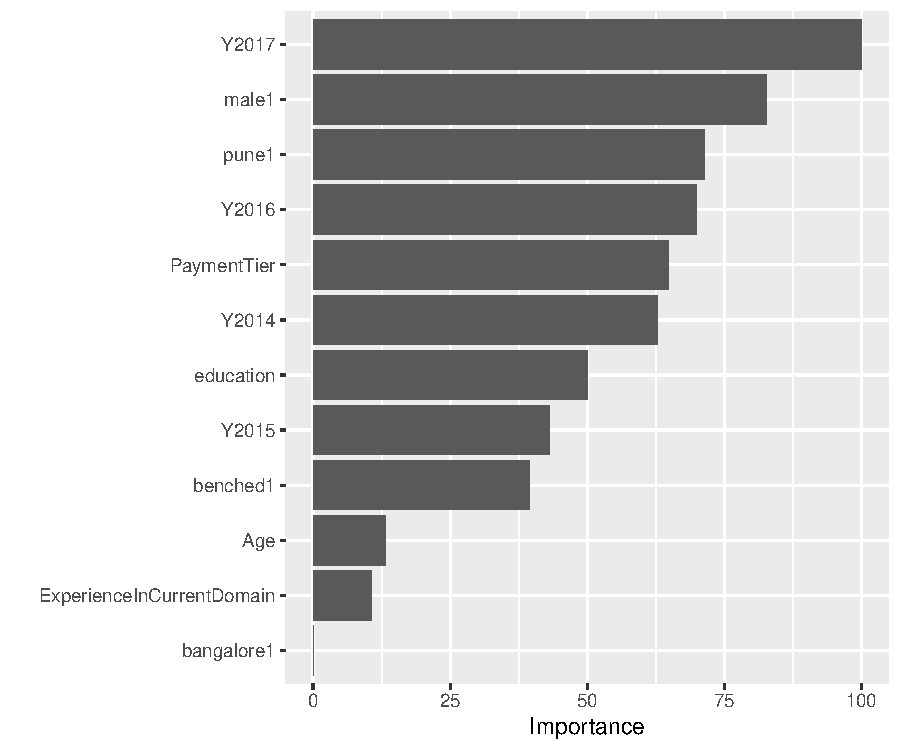
\includegraphics{Final_project_files/figure-latex/Table4-1.pdf}

In terms of the most important features, gender and the joining year of
2017 are the most important predictive features. Most of the other
variables do carry some level of importance, therefore the model is not
overly reliant on gender and joining year. This also provides an
indication that the variance of the model is not too high. While the
model suffers some level of bias, given that the accuracy is the model
is approximately 74 percent, it does not suffer from high bias.

The disadvantage to logistic models is that they assume linearity. It is
plausible that there are some nonlinear relationships between employee
attributes and attrition. Given that KNN and Random Forests are better
equipped to handle more complex problems, these models are evaluated in
the subsequent sections.

\hypertarget{knn}{%
\section*{KNN}\label{knn}}
\addcontentsline{toc}{section}{KNN}

The K-nearest neighbour (KNN) algorithm predicts each observation based
on its similarity to other observations. It identifies ``k''
observations that are most similar to the new record being predicted and
uses the most common class of those k observations as the predicted
output (Boehmke and Greenwell, 2019).

Using the KNN approach, a grid-search is conducted to find the optimal
level of K. Low values of K makes the model sensitive to noise and less
generalisable while large values can lead to oversmoothing (Boehmke and
Greenwell, 2019).

The accuracy metric is used to find the optimal value for K, given that
is an appropriate metric for a classification problem. The grid search
uses cross-validation techniques to looks for the optimal level of K
between 2 and 25. The model selects k =6 as the optimal value. The
accuracy rate for k=6 is 85\% on the training data. For the testing
data, the model's accuracy is slightly lower at 83\%. This is a
substantial improvement compared to the logistic model.

Alongside the model's accuracy, the precision, recall and F1 score are
also examined and presented in Table 1.8. The precision is 85\%, which
is relatively high. This indicates the model is good at predicting
positive outcomes. The recall, however, is much lower (60\%). This
indicates that the model has a higher false negative rate than false
positive rate, and is not as good at predicting negative outcomes.

The F1 score for the optimal K-nearest neighbours model is 70\%,
indicating that the model is adequate. These metrics all dominate the
logistic regression, indicating that the KNN model performs better.

\begin{table}[H]
\centering
\begin{tabular}{rlll}
  \hline
 & Reference & Prediction & Count \\ 
  \hline
1 & 1 & 1 & 281 \\ 
  2 & 1 & 0 &  46 \\ 
  3 & 0 & 1 & 199 \\ 
  4 & 0 & 0 & 870 \\ 
   \hline
\end{tabular}
\caption{Confusion Matrix for KNN Model \label{tab1}} 
\end{table}

\begin{table}[H]
\centering
\begin{tabular}{rlr}
  \hline
 & Metric & Value \\ 
  \hline
1 & Accuracy & 0.83 \\ 
  2 & F1 Score & 0.70 \\ 
  3 & Recall & 0.60 \\ 
  4 & Precision & 0.85 \\ 
   \hline
\end{tabular}
\caption{Metrics for KNN Model \label{tab1}} 
\end{table}

\begin{table}[H]
\centering
\begin{tabular}{rlr}
  \hline
 & Metric & Value \\ 
  \hline
1 & Training Accuracy & 0.85 \\ 
  2 & Test Accuracy & 0.83 \\ 
  3 & Training Error & 0.15 \\ 
  4 & Test Error & 0.17 \\ 
   \hline
\end{tabular}
\caption{More Metrics for KNN Model \label{tab1}} 
\end{table}

Overall, the KNN performs well in predicting employee attrition and is
useful for this particular classification problem. However, KNN models
are very sensitive to feature scaling. Results can easily become biased
as variables with larger scales can dominate the distance to
calculation. Random forests, on the other hand, are generally more
robust, especially when dealing with outliers or noise in the data. As a
result, random forests are examined in the following section for
comparison.

\hypertarget{random-forests}{%
\section*{Random Forests}\label{random-forests}}
\addcontentsline{toc}{section}{Random Forests}

Random forests are powerful out-of-the-box algorithms that generally
have very good predictive accuracy (Boehmke and Greenwell, 2019). They
combine multiple decision trees to make predictions. One key feature of
random forests is their ability to mitigate tree correlation and reduce
instability. In sum, random forests are associated with improved
performance and model robustness.

Once again, the data follows a 70:30 split between training and test
data.

\hypertarget{decision-tree}{%
\subsection*{Decision tree}\label{decision-tree}}
\addcontentsline{toc}{subsection}{Decision tree}

For illustrative purposes a single decision tree is plotted below and
its accuracy is examined. In this instance, the root node is whether or
not an employee joined in 2018. If they did not join in 2018, the tree
spits into interior nodes relating to payment tier, education, and
gender, among others to make its prediction.

Decision trees typically lack predictive performance. However, in this
instance the accuracy rate is 82\%.

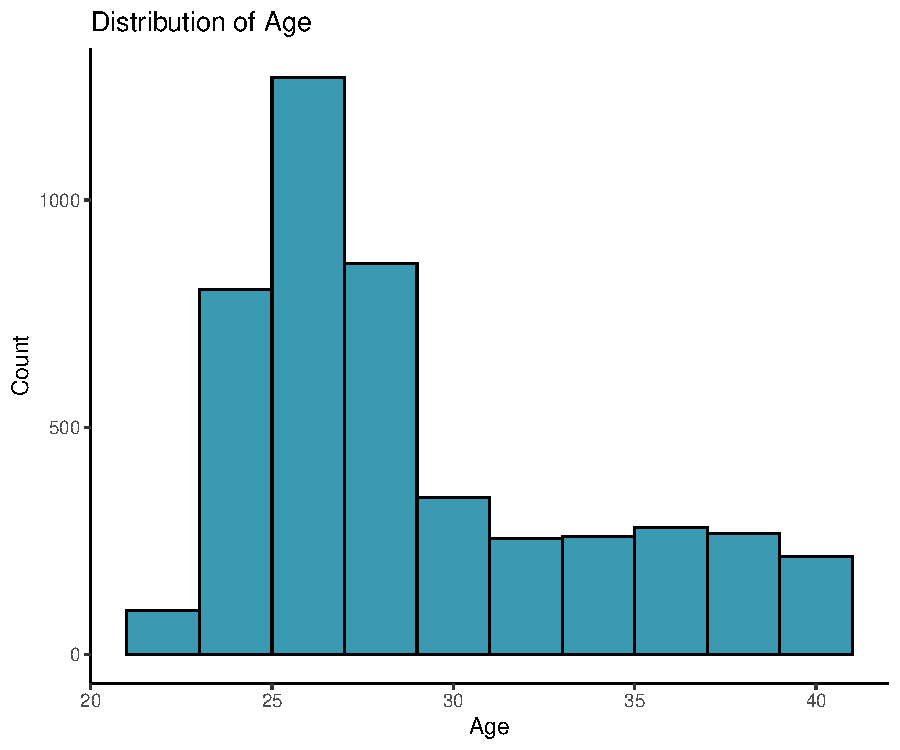
\includegraphics{Final_project_files/figure-latex/unnamed-chunk-4-1.pdf}

\hypertarget{baseline-random-forest}{%
\subsection{Baseline Random Forest}\label{baseline-random-forest}}

To enhance predictive power, the results from the baseline random forest
are presented below. In the baseline model, number of trees are set to
500 by default. The m(try) parameter is set to the square root of the
number of parameters, given that this standard when investigating a
classification problem. The default node size is 1 and the default
sampling scheme is one with replacement.

\begin{table}[H]
\centering
\begin{tabular}{rlll}
  \hline
 & Reference & Prediction & Count \\ 
  \hline
1 & 1 & 1 & 308 \\ 
  2 & 1 & 0 & 172 \\ 
  3 & 0 & 1 &  23 \\ 
  4 & 0 & 0 & 893 \\ 
   \hline
\end{tabular}
\caption{Confusion Matrix for Baseline Random Forest \label{tab1}} 
\end{table}

\begin{table}[H]
\centering
\begin{tabular}{rlr}
  \hline
 & Metric & Value \\ 
  \hline
1 & Accuracy & 0.85 \\ 
  2 & F1 Score & 0.74 \\ 
  3 & Recall & 0.61 \\ 
  4 & Precision & 0.94 \\ 
  5 & AUC ROC & 0.80 \\ 
   \hline
\end{tabular}
\caption{Metrics for Baseline Random Forest \label{tab1}} 
\end{table}

In terms of accuracy, the model's accuracy on the training data is 87\%,
compared to 85\% on the test data.Comparing the training and testing
error, the test error (15.1\%) is slightly higher than the training
error (13\%). This may indicate that there is some level of overfitting,
given that the training data performs better, however it does not appear
to be substantial.

In terms of other metrics, the F1 score is high at 74\% indicating that
the model's performance is overall very good. The precision and recall
indicate that the model is again better at predicting positive outcomes
than negative outcomes. A metric for area under the ROC curve is also
included. The ROC compares the sensitivity and specificity of the model.
As the area under the curve is 80\%, this indicates that the overall
predictive performance of the model is good and the model is reliable
for this classification task. The model is effective in distinguishing
between between the two classes of whether an employee leaves or not.

\begin{table}[H]
\centering
\begin{tabular}{rlr}
  \hline
 & Metric & Value \\ 
  \hline
1 & Training Accuracy & 0.87 \\ 
  2 & Test Accuracy & 0.85 \\ 
  3 & Training Error & 0.13 \\ 
  4 & Test Error & 0.15 \\ 
   \hline
\end{tabular}
\caption{More Metrics for Baseline Random Forest \label{tab1}} 
\end{table}

\hypertarget{hyper-parameter-tuned-random-forest}{%
\subsection{Hyper-parameter Tuned Random
Forest}\label{hyper-parameter-tuned-random-forest}}

Although the baseline model performed well, there are several
hyper-parameters to consider and adjust in this model, including the
number of trees, the number of features to consider at a given split,
the complexity of each tree, the sampling scheme, and the splitting rule
to use during tree construction. The model hyperparameters are adjusted
to achieve the best mix of bias and variance.

Following the baseline random forest model, a grid search is conducted
over a range of hyperparameters in an attempt to select the optimal
model.

Regarding number of trees, the grid search compares models with 100, 150
and 250 trees. Given that there are 15 variables, the rule of thumb is
generally 150 trees. A range around 150 is thus investigated.

Nodes sizes of 1, 3, 5 and 10 is included in the grid search. Increasing
node size decreases tree complexity.

Sample size influences how many observations are drawn for the training
of each tree (Boehmke and Greenwell, 2019). Decreasing the sample size
leads to more diverse trees and less between-tree correlation, which has
a positive effect on predictive accuracy. Having a few features that
dominate, reducing the sample size can help reduce between-tree
correlation. In other words, smaller sample size fractions can increase
the variance of the model, risking overfitting, but lower the model's
bias. Sample fractions of 50\%, 63\% and 80\% are considered.

Having many categorical features with varying number of levels, such as
experience or education in this case, or unbalanced categories, then
sampling with replacement can lead to biased results. Sampling without
replacement can thus lead to a less biased use of all the levels across
the trees in the random forest. The default sampling scheme for a random
forest is one with replacement. As a result, the grid search compares
models with and without replacement.

To select the best model, the grid search finds the out-of-bag error for
each possible model. The model with the lowest RMSE is chosen as the
best model. Comparing the RMSE of the baseline model to the new tuned
model, the tuned model is a 1.9 percent improvement over the baseline
model.

The best model selected is one with m(try) set to 4, a number of trees
as 250, a node size of 1, sampling without replacement, and a sample
fraction of 0.63.

Although the improvements are small, training accuracy increase to 89\%
and test accuracy to 86\%. Consequently, the errors for both are overall
smaller. The area under the ROC is unchanged compared to the baseline.
The F1 score, however, rose to 77\% indicating great overall
performance.

\begin{table}[H]
\centering
\begin{tabular}{rlll}
  \hline
 & Reference & Prediction & Count \\ 
  \hline
1 & 1 & 1 & 318 \\ 
  2 & 1 & 0 & 162 \\ 
  3 & 0 & 1 &  30 \\ 
  4 & 0 & 0 & 886 \\ 
   \hline
\end{tabular}
\caption{Confusion Matrix for Tuned Random Forest \label{tab1}} 
\end{table}

\begin{table}[H]
\centering
\begin{tabular}{rlr}
  \hline
 & Metric & Value \\ 
  \hline
1 & Accuracy & 0.86 \\ 
  2 & F1 Score & 0.77 \\ 
  3 & Recall & 0.65 \\ 
  4 & Precision & 0.93 \\ 
  5 & AUC ROC & 0.80 \\ 
   \hline
\end{tabular}
\caption{Metrics for Tuned Random Forest \label{tab1}} 
\end{table}

\begin{table}[H]
\centering
\begin{tabular}{rlr}
  \hline
 & Metric & Value \\ 
  \hline
1 & Training Accuracy & 0.89 \\ 
  2 & Test Accuracy & 0.86 \\ 
  3 & Training Error & 0.11 \\ 
  4 & Test Error & 0.14 \\ 
   \hline
\end{tabular}
\caption{More Metrics for Tuned Random Forest \label{tab1}} 
\end{table}

Assessing variable importance gives an indication of the variance in the
model. If the model relies heavily on a few features, then this
indicates high variance and over-fitting. Comparing the two graphs
below, it can be seen that with impurity-based variable importance, the
model heavily relies on the joining year, specifically, those who joined
the company in 2018. This is most likely due to the high attrition rate
seen in the exploratory data analysis. Under permutation-based variable
importance, there is grater emphasis on more features such as education,
payment tier and gender, despite joining year being the most important
predictive feature.

Comparing the graphs below to the variable importance plot for the
logistic regression, the random forest model appears to suffer from
higher variance due to its heavier reliance on certain features. This
shows a clear example of the bias-variance trade-off, given the improved
accuracy of the random forest model compared to the logistic model.

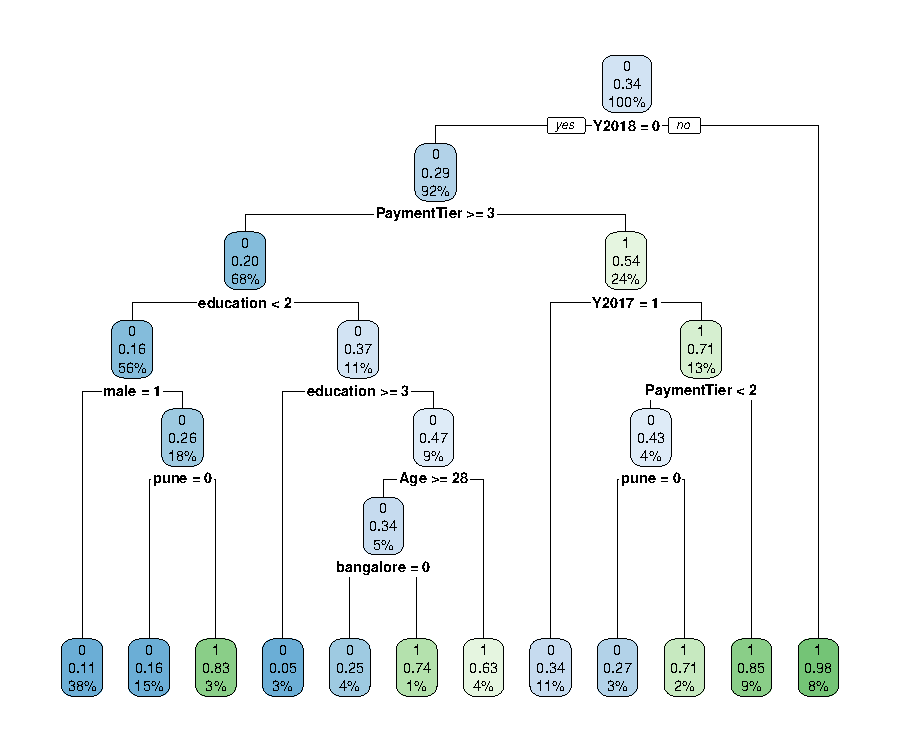
\includegraphics{Final_project_files/figure-latex/unnamed-chunk-11-1.pdf}

\hfill

\hypertarget{conclusion}{%
\section*{Conclusion}\label{conclusion}}
\addcontentsline{toc}{section}{Conclusion}

In order to predict employee attrition, various models and their
accuracy levels are assessed. The logistic regression model was
effective in predicting attrition, with the full model achieving an
accuracy rate of 71\% on the test data. However, the model showed a bias
towards false negatives. On the other hand, the K-Nearest Neighbors
(KNN) model outperformed logistic regression, with an accuracy rate of
83\% on the test data.

The best model in predicting employee attrition is the random forest
model after hyperparameter tuning. This model achieves an accuracy rate
of 86 percent against the test data. It performs well on all metrics
and, despite slight over-fitting, the model has good generalisability to
testing data.

Therefore, it is recommended that the company at hand employ this tuned
random forest model for future predictions of employee attrition rates
in order to forecast future turnover and its associated risks and costs,
as well as attempt to combat these high attrition rates.

\newpage

\hypertarget{references}{%
\section*{References}\label{references}}
\addcontentsline{toc}{section}{References}

Boehmke, B. and Greenwell, B.M., 2019. Hands-on machine learning with R.
CRC press.

\bibliography{Tex/ref}





\end{document}
